% \documentclass[table]{beamer}
\documentclass[table,handout]{beamer}
\setbeameroption{show notes}
% \setbeameroption{hide notes}
% \setbeameroption{show only notes}
\usepackage{varwidth}

\newif\ifhide
\newif\ifpost
\newif\ifhideclicker

% \hidetrue
% \hideclickertrue
% \posttrue

\newcommand{\whiteout}[1]{\textcolor{white}{#1}}
% \newcommand{\whiteoutbox}[1]{\fcolorbox{white}{white}{\parbox{\dimexpr \linewidth-2\fboxsep-2\fboxrule}{\whiteout{#1}}}}
% \newcommand{\notebox}[1]{\fcolorbox{blue}{white}{\parbox{\dimexpr \linewidth-2\fboxsep-2\fboxrule}{#1}}}
\newcommand{\whiteoutbox}[1]{\fcolorbox{white}{white}{\parbox{\linewidth}{\whiteout{#1}}}}
\newcommand{\notebox}[1]{\fcolorbox{blue}{white}{\parbox{\linewidth}{#1}}}
\newcommand{\blankbox}[1]{\phantom{\varwidth{\linewidth}\whiteoutbox{#1}\endvarwidth}}
\newcommand{\blank}[1]{\phantom{\varwidth{\linewidth}#1\endvarwidth}}

\ifhide%
    \newcommand{\hmask}[1]{\blank{#1}}%
\else%
    \newcommand{\hmask}[1]{#1}%
\fi

\ifhide%
    \newcommand{\wout}[1]{\whiteout{#1}}%
\else%
    \newcommand{\wout}[1]{#1}%
\fi

\ifhide%
    \newcommand{\hignore}[1]{}%
\else%
    \newcommand{\hignore}[1]{#1}%
\fi

\ifpost%
    \newcommand{\nopost}[1]{}%
\else%
    \newcommand{\nopost}[1]{#1}%
\fi

\ifhideclicker%
    \newcommand{\clickerslide}[1]{\stepcounter{clickerQuestionCounter}%
        \begin{frame}[t]
            \textcolor{blue}{Q \arabic{clickerQuestionCounter}:}
        \end{frame}}
\else%
    \newcommand{\clickerslide}[1]{#1}%
\fi

\ifhide%
    \newcommand{\hidebox}[1]{\blank{#1}}%
\else%
    \newcommand{\hidebox}[1]{\notebox{#1}}%
\fi

\ifhide%
    \newcommand{\wbox}[1]{\whiteoutbox{#1}}%
\else%
    \newcommand{\wbox}[1]{\notebox{#1}}%
\fi

\ifhide%
    \newcommand{\nbox}[1]{\blankbox{#1}}%
\else%
    \newcommand{\nbox}[1]{\notebox{#1}}%
\fi

\ifhideclicker%
    \newcommand{\clickeranswer}[1]{#1}%
\else%
    \ifhide%
        \newcommand{\clickeranswer}[1]{#1}%
    \else%
        \newcommand{\clickeranswer}[1]{\textbf{\textcolor{blue}{#1}}}%
    \fi
\fi

\usepackage{beamerthemesplit}
% \usetheme{boxes}
\usetheme{Malmoe}
\usecolortheme{seahorse}
% \usecolortheme{seagull}
\usepackage{ifthen}
\usepackage{xspace}
\usepackage{multirow}
\usepackage{multicol}
\usepackage{booktabs}
\usepackage{xcolor}
\usepackage{wasysym}
\usepackage{comment}
\usepackage{hyperref}
\hypersetup{pdfborder={0 0 0}, colorlinks=true, urlcolor=blue, linkcolor=blue, citecolor=blue}
\usepackage{changepage}
\usepackage[compatibility=false]{caption}
\captionsetup[figure]{font=scriptsize, labelformat=empty, textformat=simple, justification=centering, skip=2pt}
\usepackage{tikz}
\usetikzlibrary{trees,calc,backgrounds}

\usepackage[bibstyle=joaks-slides,maxcitenames=3,mincitenames=1,backend=biber]{biblatex}

\newrobustcmd*{\shortfullcite}{\AtNextCite{\renewbibmacro{title}{}\renewbibmacro{in:}{}\renewbibmacro{number}{}}\fullcite}

\newrobustcmd*{\footlessfullcite}{\AtNextCite{\renewbibmacro{title}{}\renewbibmacro{in:}{}}\footfullcite}

% Make all footnotes smaller
% \renewcommand{\footnotesize}{\scriptsize}

\definecolor{myGray}{gray}{0.9}
\colorlet{rowred}{red!30!white}

\setbeamertemplate{blocks}[rounded][shadow=true]

\setbeamercolor{defaultcolor}{bg=structure!30!normal text.bg,fg=black}
\setbeamercolor{block body}{bg=structure!30!normal text.bg,fg=black}
\setbeamercolor{block title}{bg=structure!50!normal text.bg,fg=black}

\newenvironment<>{varblock}[2][\textwidth]{%
  \setlength{\textwidth}{#1}
  \begin{actionenv}#3%
    \def\insertblocktitle{#2}%
    \par%
    \usebeamertemplate{block begin}}
  {\par%
    \usebeamertemplate{block end}%
  \end{actionenv}}

\newenvironment{displaybox}[1][\textwidth]
{
    \centerline\bgroup\hfill
    \begin{beamerboxesrounded}[lower=defaultcolor,shadow=true,width=#1]{}
}
{
    \end{beamerboxesrounded}\hfill\egroup
}

\newenvironment{onlinebox}[1][4cm]
{
    \newbox\mybox
    \newdimen\myboxht
    \setbox\mybox\hbox\bgroup%
        \begin{beamerboxesrounded}[lower=defaultcolor,shadow=true,width=#1]{}
    \centering
}
{
    \end{beamerboxesrounded}\egroup
    \myboxht\ht\mybox
    \raisebox{-0.25\myboxht}{\usebox\mybox}\hspace{2pt}
}

\newenvironment{mydescription}{
    \begin{description}
        \setlength{\leftskip}{-1.5cm}}
    {\end{description}}

\newenvironment{myitemize}{
    \begin{itemize}
        \setlength{\leftskip}{-.3cm}}
    {\end{itemize}}

% footnote without a marker
\newcommand\barefootnote[1]{%
  \begingroup
  \renewcommand\thefootnote{}\footnote{#1}%
  \addtocounter{footnote}{-1}%
  \endgroup
}

% define formatting for footer
\newcommand{\myfootline}{%
    {\it
    \insertshorttitle
    \hspace*{\fill} 
    \insertshortauthor, \insertshortinstitute
    % \ifx\insertsubtitle\@empty\else, \insertshortsubtitle\fi
    \hspace*{\fill}
    \insertframenumber/\inserttotalframenumber}}

% set up footer
\setbeamertemplate{footline}{%
    \usebeamerfont{structure}
    \begin{beamercolorbox}[wd=\paperwidth,ht=2.25ex,dp=1ex]{frametitle}%
        % \Tiny\hspace*{4mm}\myfootline\hspace{4mm}
        \tiny\hspace*{4mm}\myfootline\hspace{4mm}
    \end{beamercolorbox}}

% remove navigation bar
\beamertemplatenavigationsymbolsempty

\makeatletter
    \newenvironment{noheadline}{
        \setbeamertemplate{headline}[default]
        \def\beamer@entrycode{\vspace*{-\headheight}}
    }{}
\makeatother

\newcounter{clickerQuestionCounter}
\ifhideclicker%
\newenvironment{clickerquestion}
{ \stepcounter{clickerQuestionCounter}
  \begin{enumerate}[Q \arabic{clickerQuestionCounter}:]\color{white} }
{ \end{enumerate} }
\else%
\newenvironment{clickerquestion}
{ \stepcounter{clickerQuestionCounter}
  \begin{enumerate}[Q \arabic{clickerQuestionCounter}:] }
{ \end{enumerate} }
\fi

\ifhideclicker%
\newenvironment{clickeroptions}
{ \begin{enumerate}[\begingroup\color{white} 1)\endgroup]\color{white} }
{ \end{enumerate} }
\else%
\newenvironment{clickeroptions}
{ \begin{enumerate}[\begingroup\color{red} 1)\endgroup] }
{ \end{enumerate} }
\fi


\tikzstyle{centered} = [align=center, text centered, font=\sffamily\bfseries]
\tikzstyle{skip} = [centered, inner sep=0pt, fill]
\tikzstyle{empty} = [centered, inner sep=0pt]
\tikzstyle{inode} = [centered, circle, minimum width=4pt, fill=black, inner sep=0pt]
\tikzstyle{tnode} = [centered, circle, inner sep=1pt]
\tikzset{
  % edge styles
  level distance=10mm,
  mate/.style={edge from parent/.style={draw,distance=3pt}},
  mleft/.style={grow=left, level distance=10mm, edge from parent path={(\tikzparentnode.west)--(\tikzchildnode.east)}},
  mright/.style={grow=right, level distance=10mm, edge from parent path={(\tikzparentnode.east)--(\tikzchildnode.west)}},
  % node styles
  male/.style={rectangle,minimum size=4mm,fill=gray!80},
  female/.style={circle,minimum size=4mm,fill=gray!80},
  amale/.style={male,fill=red},
  afemale/.style={female,fill=red},
}

\newcommand{\highlight}[1]{\textcolor{violet}{\textit{\textbf{#1}}}}
\newcommand{\super}[1]{\ensuremath{^{\textrm{\sffamily #1}}}}
\newcommand{\sub}[1]{\ensuremath{_{\textrm{\sffamily #1}}}}
\newcommand{\dC}{\ensuremath{^\circ{\textrm{C}}}}
\newcommand{\tb}{\hspace{2em}}
\providecommand{\e}[1]{\ensuremath{\times 10^{#1}}}
\newcommand{\myHangIndent}{\hangindent=5mm}

\newcommand{\spp}[1]{\textit{#1}}

\newcommand\mybullet{\leavevmode%
\usebeamertemplate{itemize item}\hspace{.5em}}

\makeatletter
\newcommand*{\rom}[1]{\expandafter\@slowromancap\romannumeral #1@}
\makeatother

\newcommand{\blankslide}{{\setbeamercolor{background canvas}{bg=black}
\setbeamercolor{whitetext}{fg=white}
\begin{frame}<handout:0>[plain]
\end{frame}}}

\newcommand{\whiteslide}{
\begin{frame}<handout:0>[plain]
\end{frame}}

\newcommand{\f}[1]{\ensuremath{F_{#1}}}
\newcommand{\x}[1]{X\ensuremath{^{#1}}}
\newcommand{\y}[1]{Y\ensuremath{^{#1}}}

% Population growth macros
\newcommand{\popsize}[1]{\ensuremath{N_{#1}}}
\newcommand{\popgrowthratediscrete}[1]{\ensuremath{\lambda_{#1}}}
\newcommand{\popgrowthrate}[1]{\ensuremath{r_{#1}}}
\newcommand{\ptime}{\ensuremath{t}\xspace}

\tikzset{hide on/.code={\only<#1>{\color{white}}}}
\tikzset{
    invisible/.style={opacity=0},
    visible on/.style={alt={#1{}{invisible}}},
    alt/.code args={<#1>#2#3}{%
        \alt<#1>{\pgfkeysalso{#2}}{\pgfkeysalso{#3}}
        % \pgfkeysalso doesn't change the path
    },
}

\bibliography{../bib/references}
\author[J.\ Oaks]{
    %Jamie R.\ Oaks\inst{1}
    Jamie R.\ Oaks
}
\institute[BIOL 180]{
    \inst{}%
        BIOL 180: Introductory Biology
}



\title[Genetic variation]{Sources \& extent of genetic variation}
% \date{\today}
\date{April 15, 2015}

\begin{document}

\begin{noheadline}
\maketitle
\end{noheadline}

\nopost{
\begin{noheadline}
\begin{frame}[c]
    \vspace{-6mm}
    \begin{center} 
        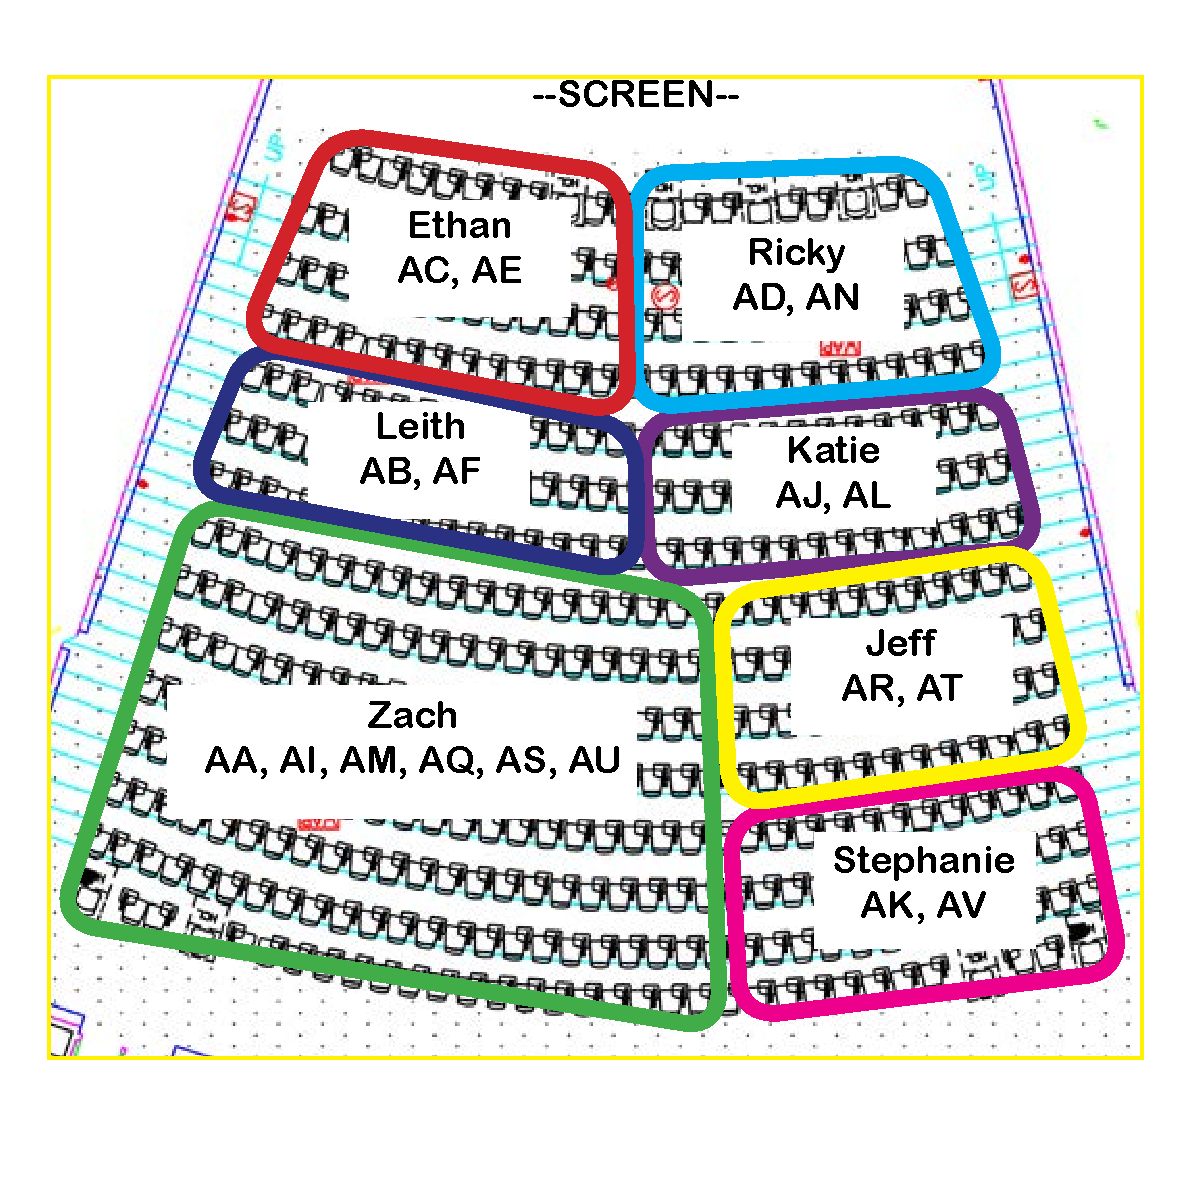
\includegraphics[height=1.3\textheight]{../images/seating-chart.pdf}
    \end{center}
\end{frame}
\end{noheadline}
}

\begin{noheadline}
\begin{frame}
\frametitle{Today's issues:}
\textbf{Why are many quantitative traits normally distributed? Where does
    genetic variation come from? Why did sex evolve?} \\
\vspace{5mm}
\tableofcontents[subsectionstyle=hide]
\end{frame}
\end{noheadline}

\clickerslide{
\begin{frame}
    \begin{clickerquestion}
        \item Why has it been difficult to understand the genetic basis of
            human traits like mental illness, intelligence, and personality?
        \begin{clickeroptions}
            \item There are significant gene $\times$ environment interactions.
            \item Gene $\times$ gene interactions are common.
            \item Many genes are involved, each with many alleles present in
                most populations.
            \item It is difficult to do the necessary studies on humans. 
            \item Many of the genes involved are pleiotropic.
            \item \clickeranswer{All of the above.}
        \end{clickeroptions}
    \end{clickerquestion}
\end{frame}
}

\section{Polygenic inheritance}

\begin{frame}[t]
    \begin{adjustwidth}{-1.5em}{-1.5em}
        \textbf{Polygenic inheritance:} Why is variation in so many traits
        normally distributed?

        \vspace{2mm}
        Basic assumptions of the model:
        \uncover<2->{
        \begin{enumerate}
            \item Many genes are involved in quantitative traits.
                \vspace{4mm}
            \item The genes assort independently.
                \vspace{4mm}
            \item In a population, there are many alleles of each gene.
                \vspace{4mm}
            \item The effects of each allele add together.
        \end{enumerate}
        }
    \end{adjustwidth}
    \note[item]{First: Warm up: What is polygenic? What is normally
        distributed? What is a model?}
\end{frame}

\begin{noheadline}
\begin{frame}[t]
    \begin{adjustwidth}{-1.5em}{-1.5em}
        \vspace{-4mm}
        \centering{
            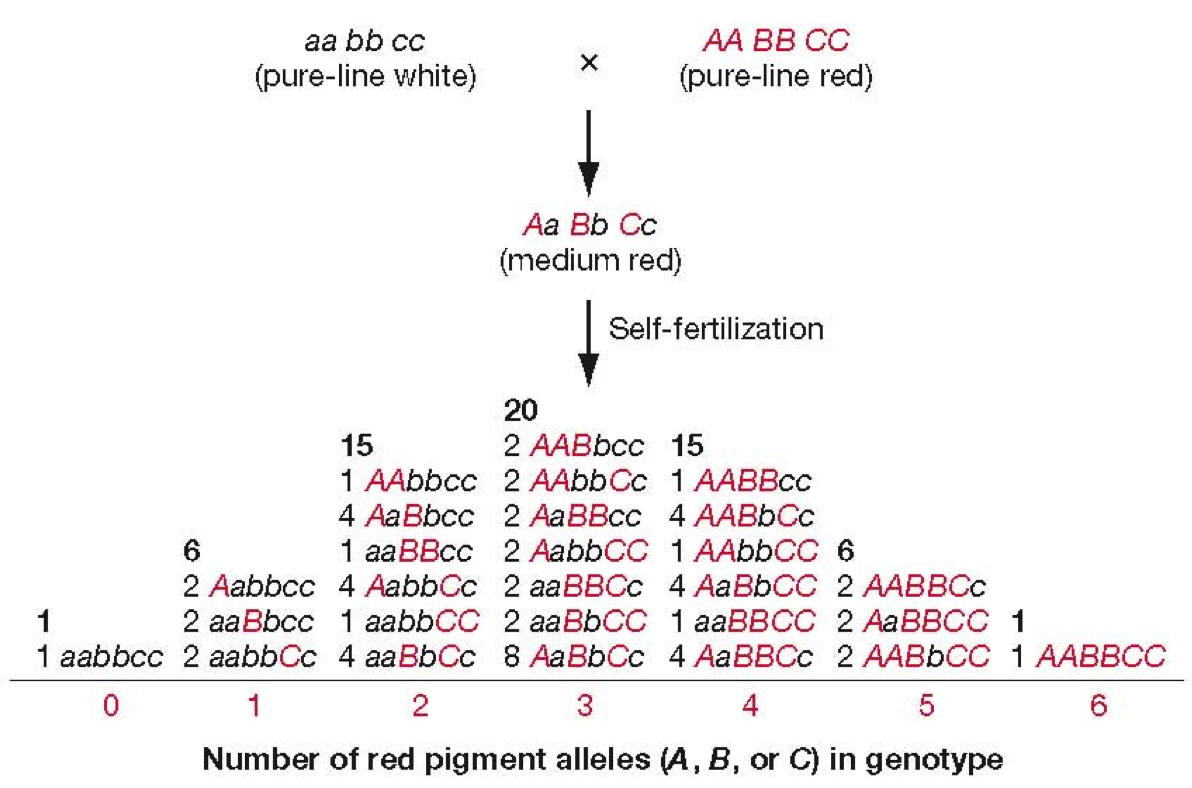
\includegraphics[width=0.8\linewidth]{quantitative-trait-histogram.png}
        }
        \uncover<2->{
        \begin{itemize}
            \item How is this different from blending inheritance? \hmask{\highlight{\small Seeing continuous variation in \f{2}s; blending predicts \f{2}s should look identical to \f{1}s}}
            \item How is this different from incomplete dominance? \hmask{\highlight{\small Incomplete dominance predicts 1 white: 2 medium red: 1 red, not continuous variation}}
        \end{itemize}
        }
    \end{adjustwidth}
    \note[item]{Kernel (seed) color in wheat; from textbook}
    \note[item]{Label Parentals, \f{1}s, \f{2}s}
    \note[item]{Model predicts normal curve, and that is what we see; strong
        evidence that model works}
\end{frame}
\end{noheadline}

\clickerslide{
\begin{frame}
    \begin{clickerquestion}
        \item It turns out that
            (1) most quantitative traits are due to the action of dozens of genes
            (2) some of these genes have much larger effects than others, and
            (3) their effects may not be additive (there can be gene $\times$
            gene interactions).
            Which conclusion from the simple model we just reviewed is still valid?
        \begin{clickeroptions}
            \item \clickeranswer{Quantitative variation in traits results from
                    the action of many genes.}
            \item Each of the three genes involved in quantitative traits adds
                an equal amount to the individual's phenotype.
            \item Quantitative traits are ``genetically determined''---meaning
                the environment has no affect on them.
            \item Almost all quantitative variation is due to variation in the
                environments experienced by individuals.
        \end{clickeroptions}
    \end{clickerquestion}
    \note[item]{Define quantitative trait---continuously varying trait
        (polygenic inheritance leads to this)}
\end{frame}
}

{
\usebackgroundtemplate{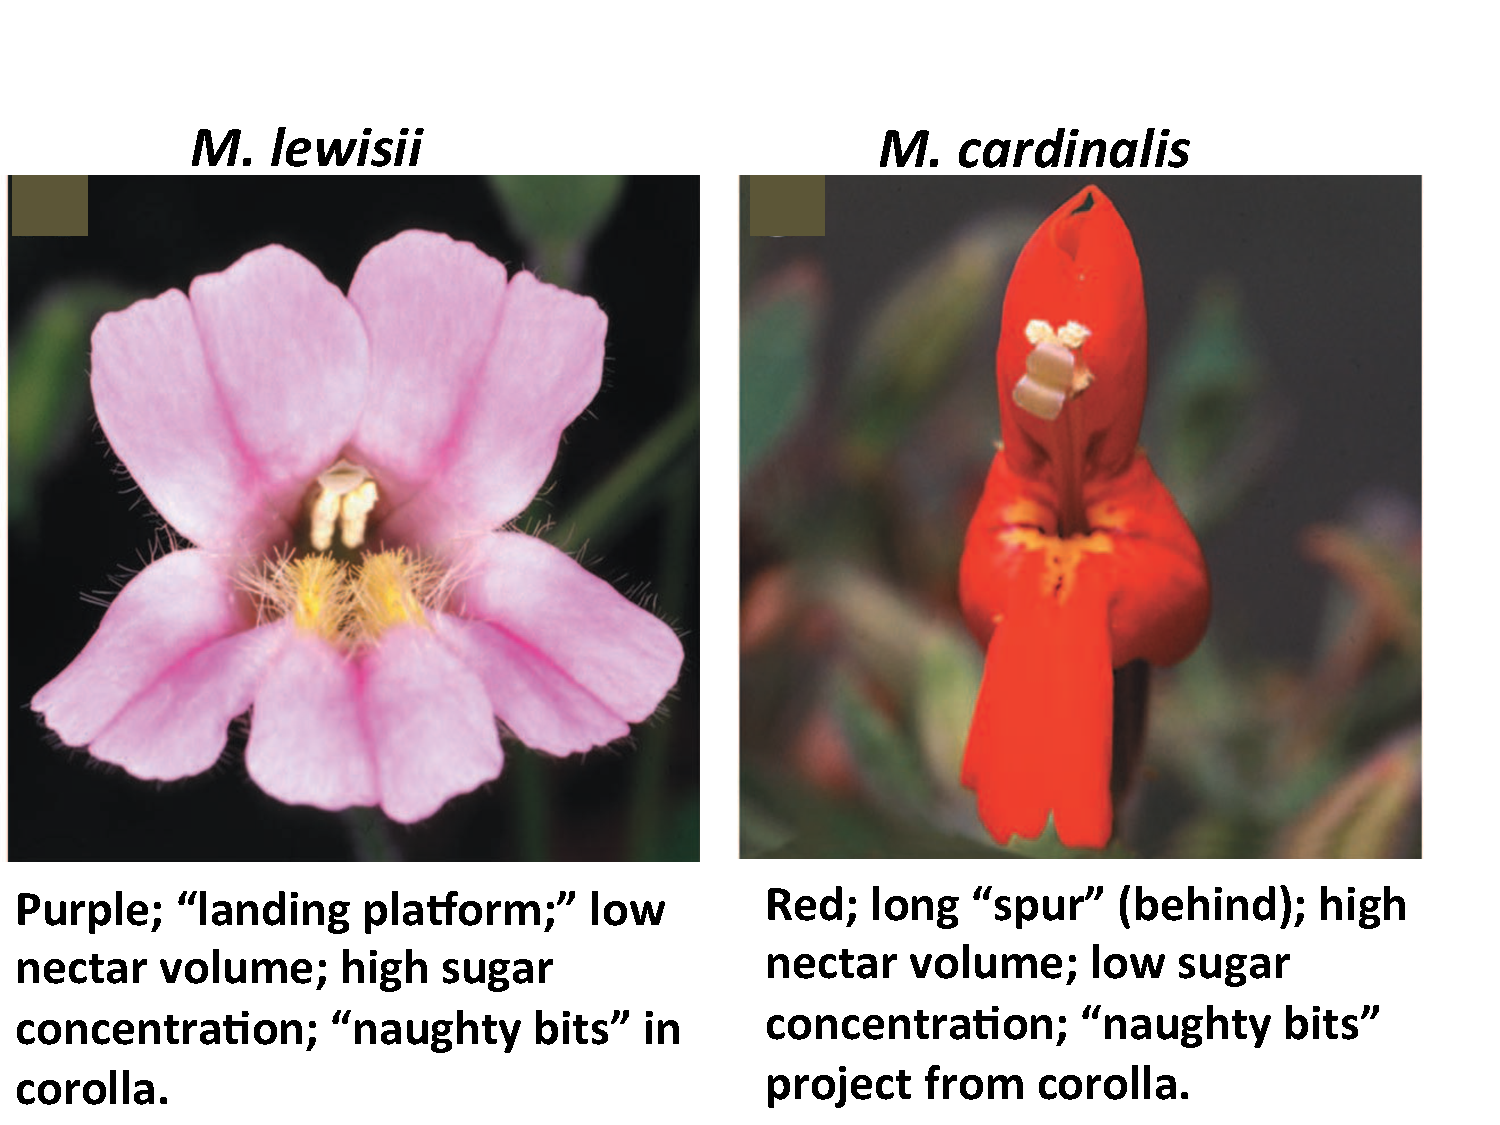
\includegraphics[page=1,width=\paperwidth]{./mimulus.pdf}}
\begin{frame}[plain]
    \note[item]{Go DAWGS! Dr. Toby Bradshaw}
    \note[item]{\textit{M.\ lewisii} pollinated by bumblebees. See purple and
        UV well, land, and enter the flower to interact with ``naughty bits'';
        nectar volume low and concentrated.}
    \note[item]{\textit{M.\ cardinalis} pollinated by hummingbirds. They see
        red well, hover (don't land), and drink a lot.}
\end{frame}
}
{
\usebackgroundtemplate{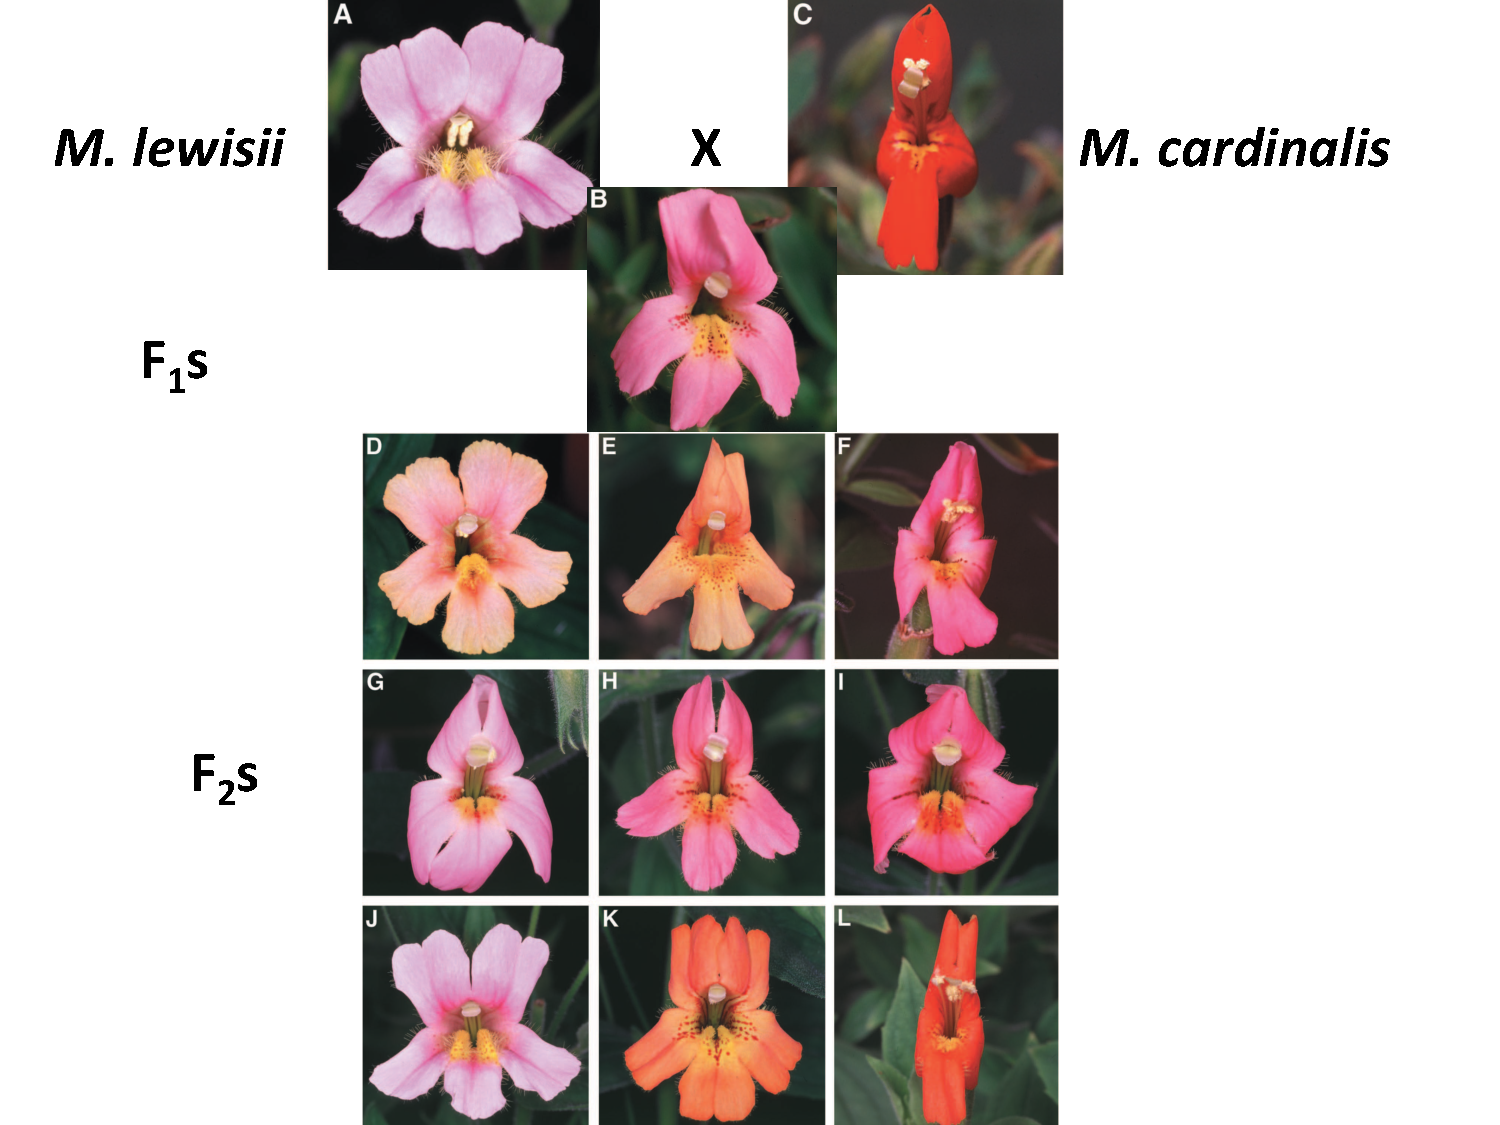
\includegraphics[page=1,width=\paperwidth]{./mimulus-cross.pdf}}
\begin{frame}[plain]
    \note[item]{\f{1}s: why?}
    \note[item]{\f{2}s: why?}
\end{frame}
}

\begin{frame}[t]
    \begin{adjustwidth}{-1.5em}{-1.5em}
        Dr.\ Bradshaw's group planted \f{2}s at random locations in natural
        habitat in the Sierra Nevada Mountains, and then recorded the type and
        frequency of pollinators that visited each flower.
        \begin{enumerate}
            \item Circle the individuals that had the most visits from
                bumblebees.

                \nbox{The ones most similar to pure \textit{M.\ lewisii} (D \&
                    J)}

            \item Put a star next to the individuals that had the most visits
                from hummingbirds.

                \nbox{The ones most similar to pure \textit{M.\ cardinalis} (F
                    \& L)}
        \end{enumerate}
        \barefootnote{\shortfullcite{Schemske1999}}
    \end{adjustwidth}
\end{frame}

\clickerslide{
\begin{frame}
    \begin{clickerquestion}
        \item What hypothesis was being tested in the field experiment?
        \begin{clickeroptions}
            \item The \f{2} hybrids can survive in the wild.
            \item Phenotypic variation is normally distributed in \f{2}s.
            \item \clickeranswer{Pollination by bees versus hummingbirds drove
                    the evolutionary divergence of the two species.}
            \item The inheritance of nectar volume, petal color, flower width,
                and other traits is polygenic.
        \end{clickeroptions}
    \end{clickerquestion}
    \note[item]{Hint: (1) \spp{M.\ lewisii} \& \spp{M.\ cardinalis} are
        \textbf{very} closely related}
    \note[item]{Hint: (2) Why did they choose the outcome variable? (= pollinator visits)}
\end{frame}
}

\begin{frame}[t]
    \begin{adjustwidth}{-1.5em}{-1.5em}
        Note: each of the key traits (nectar volume, petal color, etc.) is
        normally distributed \highlight{WITHIN} \spp{M.\ lewisii} and \spp{M.\
            cardinalis}.

        \vspace{2mm}
        Next step in the research program:
        \begin{itemize}
            \item Where does all this variation come from?
        \end{itemize}
    \end{adjustwidth}
    \barefootnote{\shortfullcite{Yuan2013,Yuan2014}}
    \note[item]{They know, down to the nucleotide differences, what makes a
        flower lewisii-like or cardinalis-like}
    \note[item]{2013 paper: Find a regulatory change in a transcription factor
        that turns on anthocyanin synthesis in \spp{M.\ cardinalis}.}
\end{frame}

\section{Four sources of genetic variation}

\subsection{Mutation}

\begin{frame}[t]
    \frametitle{Four sources of genetic variation}
    \begin{adjustwidth}{-3em}{-1.5em}
        \vspace{-4mm}
        \begin{itemize}
            \item[1.]<2-> \textbf{Mutation:} Based on 2010 sequencing data from humans,
                an average gamete contains approximately 1 base-substitution
                mutation in every $10^8$ bases.

                \begin{itemize}
                    \item<3-> How many mutations is this per gamete? {\scriptsize(Haploid
                        genome = 3.4\e{9} bases)}

                        \nbox{\small $\frac{1\textrm{mutation}}{10^8\textrm{bases}}
                            \times 3.4\e{9}\textrm{bases} \approx 34 \textrm{mutations}$}

                    \item<3-> How do these mutations create genetic variation?

                        \nbox{They create new alleles, and possibly new
                            phenotypes}

                    \item<3-> When and where do these mutation occur?

                        \nbox{During chromosome replication prior to meiosis in
                            gametocytes}

                    \item<3-> What is the physical cause?

                        \nbox{\footnotesize Errors by enzymes that copy DNA}
                \end{itemize}
                \nbox{{\scriptsize Ultimate source of variation; sources 2--4 create new
                    combos of alleles introduced via mutation}}
        \end{itemize}

    \end{adjustwidth}
    \barefootnote{\shortfullcite{Lynch2010}}
\end{frame}

\subsection{Independent assortment}

\begin{frame}[t]
    \frametitle{Four sources of genetic variation}
    \begin{adjustwidth}{-1.5em}{-1.5em}
        \begin{itemize}
            \item[2.] \textbf{Independent assortment:}

                \begin{itemize}
                    \item How does it create genetic variation?

                        \nbox{Each gamete gets a random assortment of maternal
                            and paternal chromosomes (variation AMONG
                            chromosomes). A human can create $2^{23} =
                            8.39\e{6}$ unique gametes via independent
                            assortment!}

                    \item When does it occur?

                        \nbox{Metaphase of meiosis I}

                    \vspace{9mm}
                    \item What is the physical cause?

                        \nbox{Synapsed homologs line up randomly with respect to each
                            other}
                \end{itemize}
        \end{itemize}

    \end{adjustwidth}
\end{frame}

\subsection{Recombination}

\begin{frame}[t]
    \frametitle{Four sources of genetic variation}
    \begin{adjustwidth}{-1.5em}{-1.5em}
        \begin{itemize}
            \item[3.] \textbf{Recombination (crossing over):}

                \begin{itemize}
                    \item How does it create genetic variation?

                        \nbox{Crossing over creates random changes in which
                            alleles are on each homologous chromosome---end up
                            with mix of maternal and paternal sections on the
                            same chromosome! (variation WITHIN chromosomes).
                            In outcrossing (sexual) species, recombination can
                            create \emph{almost} an infinite number of unique
                            gametes!}

                    \item When does it occur?

                        \nbox{Prophase of meiosis I}

                    \vspace{9mm}
                    \item What is the physical cause?

                        \nbox{Crossing over (exchanging sections) between
                            non-sister chromatids of synapsed homologs}
                \end{itemize}
        \end{itemize}

    \end{adjustwidth}
\end{frame}

\subsection{Outcrossing}

\begin{frame}[t]
    \frametitle{Four sources of genetic variation}
    \begin{adjustwidth}{-1.5em}{-1.5em}
        \begin{itemize}
            \item[4.] \textbf{Outcrossing (versus ``selfing''):}

                \begin{itemize}
                    \item How does it create genetic variation?

                        \nbox{Combinations of chromosomes from different
                            individuals creates new combinations of alleles.}

                        \vspace{3mm}
                    \item When does it occur?

                        \nbox{Sexual reproduction (fertilization)}

                    \vspace{8mm}
                    \item What is the physical cause?

                        \nbox{Combination of haploid gametes to create a
                            diploid (or higher ploidy)}
                \end{itemize}
        \end{itemize}

        \nbox{Sex gives independent assortment and crossing over more variation
            to shuffle---tons of variation!}
    \end{adjustwidth}
\end{frame}


\section{The evolution of sex}

\begin{frame}[t]
    \frametitle{The evolution of sex}
    \begin{adjustwidth}{-1.5em}{-1.5em}
        \begin{itemize}
            \item Why go to all this trouble, just to produce offspring that
                are genetically different from each other and from their
                parents?

                \uncover<2->{
                \vspace{1mm}
                Hypotheses:
                \begin{enumerate}
                    \item Purifying selection (getting rid of deleterious alleles)
                        \nbox{Thanks to sex, some offspring will not have the
                            deleterious (low-fitness) alleles of their
                            parent(s); not possible without sex! E.g., if you have a
                            deleterious allele and can only clone yourself, all
                            of your offspring will have that deleterious
                            allele!}

                        \vspace{1mm}
                    \item Changing environment (producing high-fitness phenotypes)

                        \nbox{Sex increases the probability that at least some
                            of offspring will have higher fitness in a changed
                            environment.}
                    
                    \begin{itemize}
                        \item What aspects of the environment change so fast
                            that sex is advantageous compared to cloning?

                        \nbox{Disease!}
                    \end{itemize}

                \end{enumerate}
                }
        \end{itemize}

    \end{adjustwidth}
\end{frame}

\begin{frame}[t]
    \begin{adjustwidth}{-1.5em}{-1.5em}
        \vspace{-3mm}
        Morran et al.\ did an experiment with a species of roundworms that
        outcrosses 20\% of the time on average. They tracked the evolution of a
        population in the presence and absence of a bacterial parasite. What is
        the take-home message here?

        \centering{
            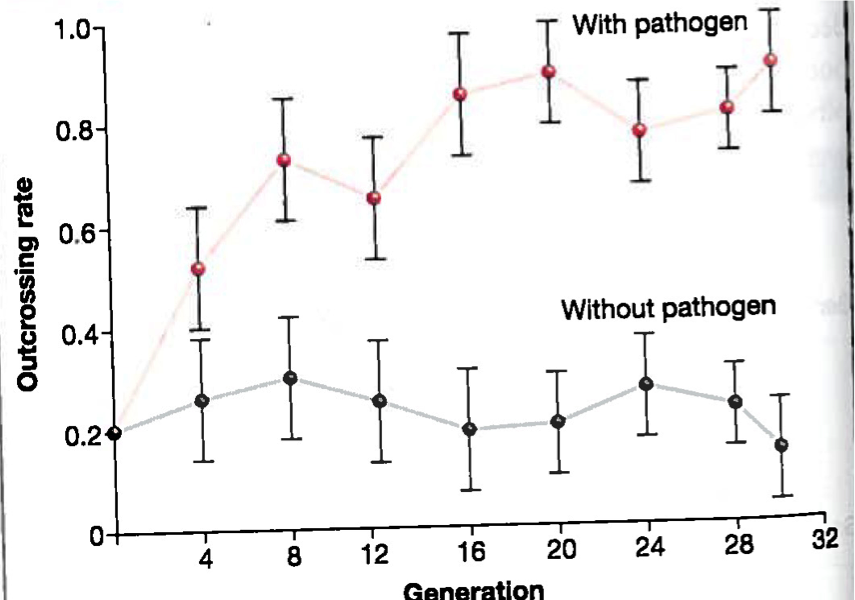
\includegraphics[height=0.6\textheight]{roundworm-outcrossing-plot.png}
        }

        \nbox{\tiny In presence of pathogen, worms that outcross more
            often have higher fitness---this supports the changing-environment
            hypothesis.}
        \vspace{-2mm}
        \barefootnote{\shortfullcite{Morran2011}}
    \end{adjustwidth}
    \note[item]{Roundworms are hermaphroditic; they can self or outcross; this
        trait has heritable variation---it can evolve!}
\end{frame}

\begin{frame}[t]
    \begin{adjustwidth}{-1.5em}{-1.5em}
        Why do college students think that t-shirts smell nice, \highlight{IF}
        they were worn by someone with different MHC alleles than they have?

        \begin{itemize}
            \item MHC = Major Histocompatibility Complex: Proteins on surfaces
                of cells that are \highlight{critical} for the immune system.
                They ``recognize'' pathogens, and ``flag them.''
        \end{itemize}
        \barefootnote{\shortfullcite{Wedekind1995}}
    \end{adjustwidth}
\end{frame}

\end{document}

\clickerslide{
\begin{frame}
    \begin{clickerquestion}
        \item 
        \begin{clickeroptions}
            \item 
            \item 
            \item 
            \item 
        \end{clickeroptions}
    \end{clickerquestion}
\end{frame}
}
